\section{Working aspects of common software}
\label{sec:processor}

In this chapter the chosen pieces of software will be put under the loop. Where the aspects each program consists of will be examined to see how they could be improved by quantum algorithms.

Lets first collect the list of software we will be examining:
\begin{itemize}
	\item Excel
	\item Google chrome
	\item Steam
	\item Counter-Strike 2
	\item Word
	\item Discord
\end{itemize}

\subsection{Excel}
In essence, Excel is an extension to a 2D array. Where the biggest extension are the formula's and the table lookup. One of the first features to highlight, which word also contains, and many of the other programs. Is the text search feature. Where you can press ctrl+f to search up a string. A string being a simple piece of text. This can be improved with a quantum algorithm for string matching \cite{QuantumStringMatching}.
\\\\
The formula's present their own form of challenge as they parse the strings input by the user into usable logic. Where the formula's are constructed into decision trees \cite{ExcelForum}. So if one set of cells is updated another cell will be recalculated. In this aspect, there are few things to "quantify". Ofcourse, as we will see with some other applications, the randomization functions can be improved. As randomization functions currently in use are not actually random. So, it could be improved by using quantum random number generation.
\\\\
Another aspect to consider are the graphs found within excel. These work by first identifying the values written, what type and what the range of the data is. It then processes this data and renders it into a graph. None of these aspects are really fit to be turned quantum. As the rending is a simple 2D rendering, which isn't that advanced that it could use quantum assistance. and neither is the range finding, data type checking and data processing. As all of these rely on simple and quick logic a majority of the time.
\\\\
The last aspect we will look at for excel will be the tables. As they work more like a database. Which is interesting, as plenty of improvements have been made to databases with quantum computing. The following has been able to be improved by quantum computing: Database searches, database manipulation, query optimization, database security and transaction management \cite{quantumDB}. Ofcourse not all of these are applicable, but for example database search and query optimization are some interesting topics. As you can also search in those tables, akin to a database.
\newpage
\subsection{Google chrome}
The all too familiar browser. There are very few people which have never interacted with one of these, where google chrome is the standard which comes pre-installed on many devices. Surprisingly, it does very little on its own. Conceptually at least, as browsers have been expanding in functionality. But they all do one thing. They call up a server via an address, ask it for the files to display and then interpret the code as a web-page. See a graph of the mechanics in Figure \ref{fig:sycamore_processor}.
\\\\
Keep in mind that a search engine is not part of the browser itself. Where the search engine is just another web-page. A web-page which is very common and where the browser automatically points to when searching, but still a web-page. 
\\\\
\begin{figure}[t]
  \centering
  \includegraphics[scale=0.5]{img/Components-of-a-browser.ps}
  \caption{Graph of how a browser works}
  \label{fig:sycamore_processor}
\end{figure}
It should be noted that the connection it makes, should be secure. Here is where quantum internet comes in. Quantum internet can send a message, a key, while knowing when someone intercepted it. A spy catcher of sorts, where the fact that q-bits collapse when read is used to the advantage of the end user's security. Besides this one thing, there are very little other known applications for a QPU in browsing. It could be possible to replace or optimize some regular code interpretation algorithms with quantum ones. But these would be case by case and would start getting very specific, so this will not be included in this paper.
\newpage
\subsection{Steam}
Surprisingly, steam has its own browser. Not just some user interface which picks up elements from the site. It is a full blown browser, which is not intended to go outside of the pages monitored by valve (the company behind steam). Besides this, it does not have a lot of extra components to it. It can download big files and install them. But both of these just rely on internet speed, which could be improved if a method of super-dense communication is found with Q-bits. But besides that? not a lot of aspects to quantify.

\subsection{Discord}
Discord, alike steam, does not have a lot of noteworthy aspects. It is an application which alike steam mostly relies on UI (user interface) and an internet connection. Meaning that it would benefit from secure communication. Which could either be done via quantum internet or encryption and decryption by a QPU for security. One more interesting aspect is how it uses a 3rd party piece of software called krisp. Which, yes, is not actually part of discord directly. But for the sake of at least giving it something, it will be included. 
\\\\
Krisp is a type of noise filtering software. When someone might be working in a noisy environment, the noise might get in the way and make them harder to hear. This is where Krisp would come into play, it filters out this background noise. It does this with an AI, this is the aspect which is where quantum could be introduced \cite{quantumai}. 

\subsection{Word}
Word is an extension to excel, surprisingly. A lot of the features used in excel are present within word. Alike the ribbon UI which can be seen at the top of both word and excel, this is a shared feature. Another is the possibility to record macro's or code them via VBA. But again, neither of these two are fit for a quantum approach. One feature which was mentioned in 3.1 is also applicable here, The text search. 
\\\\
Besides this it is also said that they are planning on integrating an AI. An AI to help with the writing of documents. Where again, an AI is something which can be improved with quantum computing.

\newpage
\subsection{Counter-Strike 2}
Here we get to some really interesting things, as games as a whole contain a lot of "smaller" aspects not often seen in other applications. At least, not directly. First of, a description of the game and how it works. 
\\\\
The game is a 3D team versus team shooter. Where you are a team of players, normally you would be on a team with 5 players when playing the most played game-mode. As the game technically is not a team versus team shooter, it does contain other game-modes. But these see lower player counts, so will be dropped in favour of analysing what could be improved in the main game-mode and to just stick to one description. 
\\\\
When you start a round, you get dropped into a map with your 4 other team-members. you get to buy a weapon, body armor and grenades with your remaining cash and then the round starts. Where the round ends by either one of the two teams dying, the timer running out or one of the two teams completing the objective. Where the teams have their own objective, one of the team plays terrorist and the other plays against them. The goal of the first team is to put down an explosive device and to defend against the other team, as the other team could defuse this device.
\\\\
The map itself consists of routes players can take to get to the locations where the device can be put down. And props, hiding locations and corners. This is how the game is to play and how it is played. 
\\\\
But the mechanics behind it function far differently. As it uses a set of things to let it seam real. First of all are all of the models, they make up crates, people, guns, everything in the game. Nearly all games work like this, they use models, or meshes in a different sense of the word. Meshes exist out of vertexes, which are points in space, where a mesh is a bunch of them connected to one another. On top of these meshes there will be textures, These show the color. As by default, a mesh would be colourless. These textures have multiple layers to them, one albedo layer, one normal layer and one roughness layer. Some could have more, but these 3 are default. The albedo is the color which can be seen, the other 2 do something special. The roughness map will be used to display how smooth and reflective one part of a mesh is, so if one part of it is white it would be reflective and if it is black it would absorb light and be darker. 
Then we have the normal map, a texture which dictates how much the GPU should render the mesh in a displacement way. It shows if a mesh should stick slightly out or if it should bend inwards. 
\\\\
That will show the models. But not actually render them to the screen, as both lighting and a rendering method are needed for that. There are multiple rendering methods, but 2 mayor types: rasterization and ray tracing. Rasterization is the most common and less computationally expensive. It transforms the triangles the vertexes make up to the screen, to the raster of pixels which make up the screen. The other method, ray tracing, is known to be computationally expensive. As this method uses light rays emitting from the camera, where those rays bounce of off the environment. These bounces will record what every pixel should look like and give a quite realistic image. But here is where we get to one of the quantum aspects. As there is technically another method of rendering in the works, a quantum one \cite{quantumRender}. This would use a QPU to render a 3D scene instead of a GPU. 
\\\\
Next up is lighting, as this is also an essential part to a map. And with light, come shadows. Shadows which are again hard to compute. Which is why earlier games would bake shadows into the textures of the maps. So it would pre-render the shadows of all meshes and add that to the albedo. But due to hardware improvements, most games will use this sparsely, instead opting for real-time shadows. So far no quantum solution has been proposed for this niche problem.
\\\\
A new technology which has been put out by Nvidia, Intel and AMD is image up-scaling. This technology uses ai to first render the game in question in a lower resolution and will use the ai to upscale this lower resolution image into a higher one. It is quickly being integrated into many games. on medium and lower end computers this technology can help a lot to lower the performance cost of the game. Nvidia has even brought out another version of this, DLSS. DLSS does not only do the upscaling stated above, it also generates frames in-between. Meaning that the computational cost is nearly halved in trade for some fidelity on the interpolated images \cite{Dlss}. Where the performance cost of the ai could be trivialized when a QPU would be introduced.
\\\\
The last topic which would be interesting to highlight is physics. As a lot of games contain it, counter strike 2 included. Granted, the need for it is minimal, as the game barely contains examples of it. Some of those sparse examples being: grenades bouncing of off surfaces and when a player dies their corpse will rag-doll. Another aspect which could be attributed to physics is the fact that more powerful guns are capable of penetrating some thinner walls. But these physics are preprogrammed, not emergent from the general physics of the game. So no, this game has no real need for physics being of lower computational cost. But, there is one catch. In one of the maps in counter strike 2, there is a destructible model where the way it falls apart is baked into the scene and not determined by how it is destroyed. If more models where to be added like this, the speed up of physics could be a reasonable feature. Currently there are no papers out on how the speed up of physics based simulation could be done. But this does not mean there will be no possible way to do so. 